\section{Introduction} \label{introduction}

\ac{XSS} is still one of the most dominant web vulnerabilites. A 2017
report showed that 50\% of websites contained at least one \ac{XSS}
vulnerability~\cite{Acunetix}. Countermeasures exist, but many of them
lack widespread deployment, and so web users are still mostly
unprotected.

Informally, the cause of \xss is a lack of input sanitization:
user-chosen data ``escapes'' into a page's template and makes its way
into the javascript engine, or modifies the DOM
unintendedly.
%
Consequently, many of the \xss defenses published so far
propose to fix the problem at the source, by properly separating the
template from the user data on the server, or by modifying
browsers~\cite{Jim:2007:DSI:1242572.1242654,Nadji:2009,Wurzinger:2009:SMX:1656360.1656379,Sundareswaran:2012:XHS:2352970.2352994}.
%
There are also similar solutions that can be implemented in the
front-end code of an application~\cite{10.1007/978-3-319-66399-9_7}.
In all cases, these technologies must be adopted by the application
software developers.

The main drawback with these approaches, from a user perspective, is
that unless application maintainers adopt these technologies
systematically, they are of little benefit, and users remain at risk
from \xss. One hindrance to their adoption is that developers may not have the
expertise necessary, or sufficient resources to implement necessary
precautions.
%As a consequence, many of the approaches cited so far
%have not seen widespread adoption, and \xss still prevails today.
The viability of services dedicated to scanning for exploits,
and the existence of a flourishing security-consulting economy is a testament
to this.


Luckily, users wishing to gain reassurance over the safety of the
sites they visit can install browser extensions to filter malicious
scripts and content. Unfortunately, these extensions achieve most of
their security by disabling functionality in the applications, which
can severely damage the usability of the
sites~\cite{Noscript,Snyder:2017:MWD:3133956.3133966}. Most sites rely
heavily on JavaScript\footnote{As early as 2012, it is used by almost
  100\% of the Alexa top 500
  sites~\cite{Stock:2017:WTI:3241189.3241265}}, and some sites offer
versions without scripts, albeit with a level of interactivity below
what users have come to expect.
% Can something be said about the dom-based XSS attacks?

Some software vendors respond to \xss when a vulnerability is
disclosed, with patches. When the software affected is released in
the form of packages, frameworks, or libraries, and used by several
web applications, there are extra delays before users can benefit from
the patch -- the updated software has to first be deployed by service
administrators.

Unfortunately, website administrators will not, and often cannot,
apply software updates immediately: one study found
that 61\% of WordPress websites were running a version with known
security vulnerabilities~\cite{Sucuri}. In another report, we learn
that 30.95\% of Alexa's top 1 Million sites run a vulnerable version
of WordPress~\cite{wpwhitesecurity}.

Users are in effect at the mercy of developers and administrators if
they need to browse safe, up-to-date, applications. Our solution \sys,
remedies this problem -- based on a database of known vulnerabilities,
it aims to patch any vulnerable page displayed in the user's browser.

\begin{figure}[h]
  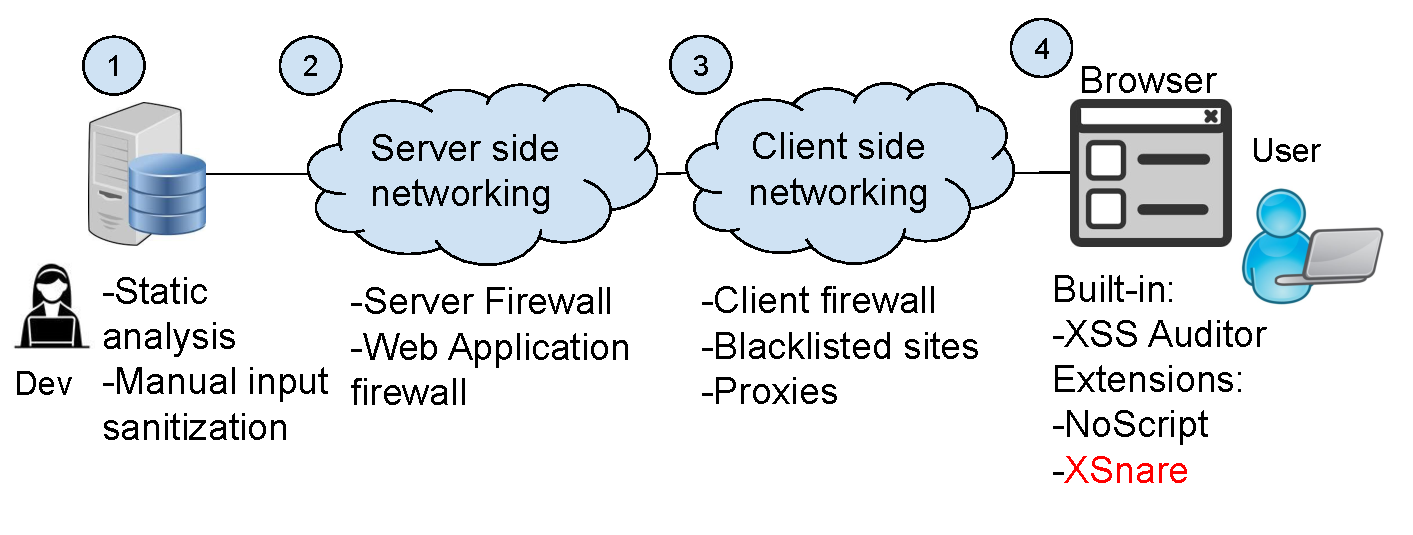
\includegraphics[scale=0.37]{img/web_app_architecture_one.pdf}
  \vspace*{-5.0ex}
%  \caption{Architecture of typical web applications. Different security solutions apply at distinct layers.}
  \caption{Different web security solutions with XSnare on the client-side.}
  \label{fig:web_architecture}
\end{figure}

Each layer of the web application stack  (Figure~\ref{fig:web_architecture}) opens different defence options against \xss:
%Further details of these different approaches are described in Section 5:
\begin{enumerate}

\item The application logic is the first line of defence.
  Code safety can be enhanced with third-party vulnerability scanning solutions, and a thorough
  code-review process. Taint, and static code analysis tools can detect unsanitised inputs.

\item In the hosting environment, network firewalls, specifically \acp{WAF} can defend against attacks such as \ac{DDoS}, \ac{SQL} injections and \ac{XSS}.

\item In the client's environment (residential or commercial), users may install network firewalls, network content filters, and web proxies.

\item The last line of defence is the browser.
  Browser have built-in defences, such as
  Chrome's \ac{XSS} Auditor~\cite{xssauditor}. Users can also
  install third-party extensions to block malicious requests and
  responses, such as NoScript~\cite{Noscript}, and \sys.
\end{enumerate}

We draw two observations from existing solutions, a) server-side
solutions have to be applied independently on each server, and b)
solutions on the client are typically written as generic filters which
catch everything, and consequently do not take full advantage
of the specificity of an application or vulnerability.

For example, a \ac{WAF} can effectively protect the deployment placed
behind it, but users cannot realistically expect that every site they
visit be protected by one. At the opposite end, in the client's
environment, a user might configure a network proxy for all website
traffic, with generic rules achieving maximum coverage, but this
will often lead to an elevated rate of false positives (FPs).

Similarly, browser built-in defences are very coarse, and will only
work on a subset of exploits. Chrome's XSS Auditor, for example, only
attempts to defend against reflected \ac{XSS}. Google recently
announced its intention to deprecate XSS Auditor, for reasons
including \emph{``Bypasses abound''}, \emph{``It prevents some legit
  sites from working''}, and \emph{``Once detected, there's nothing
  good to do''}~\cite{deprecatexssauditor}. Stock et
al.~\cite{precise_dom_xss} propose enhancements to XSS Auditor and
cover a wider range of exploits than the auditor, but are limited to
DOM-based \ac{XSS}.  Our work covers all types of \ac{XSS}.

Implementing adequate server-side protections~\cite{Xu:2006:TPE:1267336.1267345,DBLP:conf/sec/Nguyen-TuongGGSE05,Pietraszek:2005:DAI:2146257.2146267,Bisht:2008:XPD:1428322.1428325} throughout a codebase could arguably qualify as a colossal task, considering the high turnaround times for resolving simpler bugs. A 2018 study found that the average time to patch a \ac{CVE}, all severities combined, is 38 days, increasing to as much as 54 days for low severity ones, and the oldest unpatched \ac{CVE} was 340
days old~\cite{Rapid7}.

%% % JS: I think this is false (or unproven, anyway):
% A client-side solution does not rely on application developers, so it reduces the turnaround time between a vulnerability and its patch.

%% IB: Cut for space.
%%
%% Furthermore, it is
%% complementary to the aforementioned techniques: a \ac{WAF} will not reduce
%% the security of a client-side approach, and having these
%% two work in tandem is beneficial to the user's experience.

Server-side defences also do not protect against client-only forms of
\xss, e.g., reflected \ac{XSS}, or persistent
client-side \ac{XSS}, which use a browser's local storage or cookies
as an attack vector. Steffens et
al.~\cite{DBLP:conf/ndss/SteffensRJS19} present a study of Persistent
Client-Side \ac{XSS} across popular websites and find that as many as
21\% of the most frequented web sites are vulnerable to these attacks.
%% While some of these exploits are harder to carry out in practice, as
%% many as 6\% of these sites are vulnerable to an attack by a realistic
%% attacker.
%
\textbf{To provide users with the means to protect themselves in the absence
of control over servers, we strongly believe that a novel client-side
solution is necessary.}

A number of existing solutions in this area also suffer from high
rates of false-positives and false-negatives. %% , due to the lack of
%% information available at the layers they operate at.
For example, NoScript~\cite{Noscript} works via domain white-listing, thus by
default, JavaScript scripts and other code will not execute. However,
not all scripts outside of the whitelist should be assumed to be
malicious. Browser-level filters like XSS Auditor work based on
general policies and can therefore incorrectly sanitize non-malicious
content.

\textbf{We posit that the DOM is the right place to mitigate XSS
  attacks as it provides a full picture of the web application.} While
most of the functionality we provide could be done by a network filter
in front of the browser, we take advantage of additional context
provided by the browser.
%
Particularly, when an exploit occurs as a result of user interactions,
like on response to a click, we
benefit from knowledge of the initiating tab to filter the
response. Previous client-side solutions have opted for detectors that were generic and site-agnostic~\cite{Kirda:2009:CCS:2639535.2639808,Jim:2007:DSI:1242572.1242654,Hallaraker:2005:DMJ:1078029.1078861}. Our work goes in the opposite direction, and tries rather to prevent precisely-defined exploits in specific applications.

If a patch for a server-side vulnerability can be ``translated'' into
an equivalent set of operations to apply on the fully formed HTML
document in the browser, then we can seize the opportunity to defend
{\em early} against exploits of that vulnerability.
%
Our extension, which has access to the user's browsing context, can
identify vulnerable pages based on a database of signatures for
previous disclosures. This way, \sys can protect users as soon as a patch
is implemented and added to its database. The client-side
patch will remain beneficial a until \textit{all} server
operators running that software have had a chance to upgrade their
deployments.
%% We detail its design in \autoref{xsnare_design}.


 A similar philosophy is adopted by the client-side firewall-based network proxy Noxes~\cite{Kirda:2009:CCS:2639535.2639808}. %%  Rules dictate the links which can be accessed by a website
%% when generating requests, and can be created both automatically and manually
%% by a user.
Unlike \sys, however, Noxes only applies generic policies based on information available at the network layer. Namely, it does not protect against
attacks invisible to the network, e.g., deleting local files.
% It motivates the need for basic customization between domain names, but not between applications.
We believe additional contextual knowledge also offers more accurate vulnerability detection.

%% IB: Cut details below -- too detailed.
%% 
%% Furthermore, they rely on websites having a small number of external
%% dynamic links to third-parties. This likely does not hold true anymore, 
%% as websites require an ever-increasing amount of dynamic content, with 
%% several interconnections with third-parties to provide features like advertisements and analytics.



%% IB: Cut the paragraph below -- too technical for intro
%%
%% XSnare consists of three components: a trusted Firefox
%% extension for interposing between the application and the DOM, a
%% periodically updated local database which maintains exploit
%% definitions and descriptions of the vulnerabilities to be targeted by
%% the extension in the form of signatures, and finally, a declarative
%% language for describing exploits, expressive enough for an user to be
%% precise about which parts of the HTML are vulnerable and how to
%% sanitize them.

%% We aim to reproduce the developer's intended server-side patch on the
%% client-side, therefore, we need to be able to determine the separation
%% between dynamic content and the static template, and pass the dynamic
%% elements to a sanitization function. We further detail XSnare's
%% mechanisms that achieve this in Section~\ref{xsnare_design}.

We evaluate our system, by
testing its efficacy against recent \ac{XSS} CVEs. CVE databases are
well-maintained and widely available sources of real-world vulnerabilities.
%They are one of the main tools
%used by developers to patch their code against known
%vulnerabilities.
Furthermore, we measure its performance overhead on page load times,
on a wide array of sites and show that it does not significantly
affect browsing experience.

Our contributions include: 
\begin{itemize}

	\item \sys: a novel client-side framework that protects
          users against XSS vulnerabilities with a database of
          signatures for these vulnerabilities, written in a
          declarative language.

	\item A mechanism to correctly isolate a vulnerable injection
          point in a web page and to apply the intended server-side
          patch on the client-side.

	\item A collection of signatures to protect users against
          real XSS CVEs (\autoref{viability}), demonstrating the practicality
          of \sys; and the evaluation of its impact on browsing (\autoref{performance}). %% , demonstrating that our tool's
          %% feasibility in practice.

\end{itemize}
